\documentclass{article}
\usepackage[utf8]{inputenc}
\usepackage{listings}
\usepackage{xcolor}
\usepackage{mathpazo}
\usepackage{geometry}
\usepackage{fancyhdr}
\usepackage{tcolorbox}
\usepackage{enumitem}
\usepackage{tikz}
\usepackage{graphicx}

% Set page margins
\geometry{margin=1in}

% Configure fancy headers
\pagestyle{fancy}
\fancyhead{}
\fancyfoot{}
\fancyhead[L]{\textit{C++ Variable Scope}}
\fancyhead[R]{\thepage}
\renewcommand{\headrulewidth}{0.4pt}

% Configure code listings
\definecolor{codegray}{rgb}{0.95,0.95,0.95}
\definecolor{codegreen}{rgb}{0,0.6,0}
\definecolor{codecomment}{rgb}{0.5,0.5,0.5}
\definecolor{codeblue}{rgb}{0,0,0.8}

\lstset{
    backgroundcolor=\color{codegray},
    commentstyle=\color{codecomment},
    keywordstyle=\color{codeblue},
    stringstyle=\color{codegreen},
    basicstyle=\ttfamily\small,
    breakatwhitespace=false,
    breaklines=true,
    captionpos=b,
    keepspaces=true,
    showspaces=false,
    showstringspaces=false,
    showtabs=false,
    tabsize=2,
    frame=single,
    language=C++
}

% Custom box styles
\newtcolorbox{conceptbox}{
    colback=blue!5,
    colframe=blue!75!black,
    fonttitle=\bfseries,
    title=Key Concept
}

\newtcolorbox{warningbox}{
    colback=red!5,
    colframe=red!75!black,
    fonttitle=\bfseries,
    title=Common Pitfall
}

\title{\Huge{\textbf{Understanding Variable Scope in C++}}\\
       \Large{A Comprehensive Guide with Examples}}
\author{Mr. Gullo}
\date{Nov, 2024}

\begin{document}

\maketitle
\tableofcontents
\newpage

\section{Introduction to Variable Scope}
Variable scope is a fundamental concept in C++ that determines where in your program a variable can be accessed. Understanding scope is crucial for:
\begin{itemize}
    \item Writing maintainable code
    \item Preventing naming conflicts
    \item Managing memory efficiently
    \item Debugging effectively
\end{itemize}

\section{Lesson 1: Function Scope and Variable Accessibility}

\begin{conceptbox}
Variables declared inside a function are only accessible within that function unless explicitly passed to other functions.
\end{conceptbox}

\subsection{Example Code}
\begin{lstlisting}
void display();
int main() {
    int a = 10;      // Local to main
    display();       // Error: Can't access 'a'
    return 0;
}
void display() {
    cout << a;       // Error: 'a' not in scope
}
\end{lstlisting}

\subsection{Key Points}
\begin{itemize}
    \item Each function has its own separate scope
    \item Variables declared in one function are invisible to others
    \item Local variables are destroyed when the function ends
\end{itemize}

\section{Lesson 2: Pass by Value}

\begin{conceptbox}
When passing variables by value, a copy is made, and modifications to the copy do not affect the original variable.
\end{conceptbox}

\subsection{Example Code}
\begin{lstlisting}
void addOne(int a) {  // 'a' is a copy
    a++;              // Modifies copy only
}
int main() {
    int a = 10;
    addOne(a);        // Original 'a' unchanged
    cout << a;        // Still prints 10
}
\end{lstlisting}

\subsection{Memory Diagram}
\begin{center}
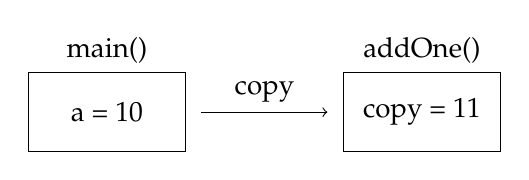
\begin{tikzpicture}
    \draw (0,0) rectangle (2,1);
    \draw (4,0) rectangle (6,1);
    \node at (1,0.5) {a = 10};
    \node at (5,0.5) {copy = 11};
    \node[above] at (1,1) {main()};
    \node[above] at (5,1) {addOne()};
    \draw[->] (2.2,0.5) -- (3.8,0.5) node[midway,above] {copy};
\end{tikzpicture}
\end{center}

\section{Lesson 3: Global Variables}

\begin{warningbox}
Global variables are accessible throughout the program but should be used sparingly as they can make code harder to maintain and debug.
\end{warningbox}

\subsection{Example Code}
\begin{lstlisting}
int a = 10;          // Global variable
void addOne() {
    a++;             // Modifies global 'a'
}
int main() {
    cout << a;       // Accesses global 'a'
    addOne();
    cout << a;       // Shows modified value
}
\end{lstlisting}

\subsection{Problems with Global Variables}
\begin{itemize}[label=$\times$]
    \item Make code harder to understand
    \item Create hidden dependencies
    \item Make testing difficult
    \item Can cause naming conflicts
\end{itemize}

\section{Lesson 4: Pass by Reference}

\begin{conceptbox}
Pass by reference allows functions to modify original variables by passing their memory address rather than making a copy.
\end{conceptbox}

\subsection{Example Code}
\begin{lstlisting}
void addOne(int& a) { // Reference parameter
    a++;              // Modifies original
}
int main() {
    int a = 10;
    addOne(a);        // 'a' will be modified
    cout << a;        // Prints 11
}
\end{lstlisting}

\subsection{Memory Diagram}
\begin{center}
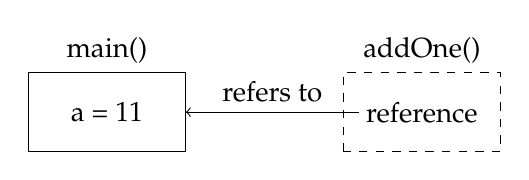
\begin{tikzpicture}
    \draw (0,0) rectangle (2,1);
    \draw[dashed] (4,0) rectangle (6,1);
    \node at (1,0.5) {a = 11};
    \node at (5,0.5) {reference};
    \node[above] at (1,1) {main()};
    \node[above] at (5,1) {addOne()};
    \draw[->] (4.2,0.5) -- (2,0.5) node[midway,above] {refers to};
\end{tikzpicture}
\end{center}

\section{Lesson 5: Variable Shadowing}

\begin{warningbox}
Variable shadowing occurs when a variable in an inner scope has the same name as a variable in an outer scope, hiding the outer variable.
\end{warningbox}

\subsection{Example Code}
\begin{lstlisting}
int a = 1;           // Global a
int main() {
    int a = 2;       // Shadows global a
    if(true) {
        int a = 3;   // Shadows main's a
    }
    cout << a;       // Prints 2
}
\end{lstlisting}

\subsection{Scope Hierarchy}
\begin{center}
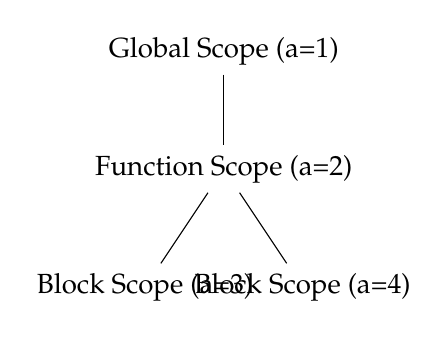
\begin{tikzpicture}[
    level distance=1.5cm,
    level 1/.style={sibling distance=4cm},
    level 2/.style={sibling distance=2cm}
]
    \node {Global Scope (a=1)}
        child {node {Function Scope (a=2)}
            child {node {Block Scope (a=3)}}
            child {node {Block Scope (a=4)}}
        };
\end{tikzpicture}
\end{center}

\section{Best Practices}

\begin{itemize}
    \item Use meaningful variable names
    \item Keep variables in the smallest needed scope
    \item Avoid global variables when possible
    \item Use pass by reference for large objects
    \item Avoid variable shadowing
    \item Document scope decisions in complex scenarios
\end{itemize}

\section{Practice Exercises}

\begin{enumerate}
    \item Identify scope issues in given code samples
    \item Convert pass by value to pass by reference
    \item Refactor code to eliminate global variables
    \item Debug scope-related problems
    \item Write functions with proper variable scope
\end{enumerate}

\begin{tcolorbox}[title=Summary]
Understanding variable scope is crucial for writing maintainable and bug-free C++ code. Remember:
\begin{itemize}
    \item Local variables are only accessible in their function
    \item Pass by value creates copies
    \item Global variables should be used sparingly
    \item Pass by reference allows modification of original variables
    \item Avoid variable shadowing
\end{itemize}
\end{tcolorbox}

\end{document}